% Options for packages loaded elsewhere
\PassOptionsToPackage{unicode}{hyperref}
\PassOptionsToPackage{hyphens}{url}
%
\documentclass[
  english,
  man]{apa6}
\usepackage{lmodern}
\usepackage{amsmath}
\usepackage{ifxetex,ifluatex}
\ifnum 0\ifxetex 1\fi\ifluatex 1\fi=0 % if pdftex
  \usepackage[T1]{fontenc}
  \usepackage[utf8]{inputenc}
  \usepackage{textcomp} % provide euro and other symbols
  \usepackage{amssymb}
\else % if luatex or xetex
  \usepackage{unicode-math}
  \defaultfontfeatures{Scale=MatchLowercase}
  \defaultfontfeatures[\rmfamily]{Ligatures=TeX,Scale=1}
\fi
% Use upquote if available, for straight quotes in verbatim environments
\IfFileExists{upquote.sty}{\usepackage{upquote}}{}
\IfFileExists{microtype.sty}{% use microtype if available
  \usepackage[]{microtype}
  \UseMicrotypeSet[protrusion]{basicmath} % disable protrusion for tt fonts
}{}
\makeatletter
\@ifundefined{KOMAClassName}{% if non-KOMA class
  \IfFileExists{parskip.sty}{%
    \usepackage{parskip}
  }{% else
    \setlength{\parindent}{0pt}
    \setlength{\parskip}{6pt plus 2pt minus 1pt}}
}{% if KOMA class
  \KOMAoptions{parskip=half}}
\makeatother
\usepackage{xcolor}
\IfFileExists{xurl.sty}{\usepackage{xurl}}{} % add URL line breaks if available
\IfFileExists{bookmark.sty}{\usepackage{bookmark}}{\usepackage{hyperref}}
\hypersetup{
  pdftitle={Reproducible Methods for Face Research},
  pdfauthor={Lisa DeBruine1 \& Iris Holzleitner1,2},
  pdflang={en-EN},
  pdfkeywords={faces; morphing; transforming; reproducible; webmorph},
  hidelinks,
  pdfcreator={LaTeX via pandoc}}
\urlstyle{same} % disable monospaced font for URLs
\usepackage{graphicx}
\makeatletter
\def\maxwidth{\ifdim\Gin@nat@width>\linewidth\linewidth\else\Gin@nat@width\fi}
\def\maxheight{\ifdim\Gin@nat@height>\textheight\textheight\else\Gin@nat@height\fi}
\makeatother
% Scale images if necessary, so that they will not overflow the page
% margins by default, and it is still possible to overwrite the defaults
% using explicit options in \includegraphics[width, height, ...]{}
\setkeys{Gin}{width=\maxwidth,height=\maxheight,keepaspectratio}
% Set default figure placement to htbp
\makeatletter
\def\fps@figure{htbp}
\makeatother
\setlength{\emergencystretch}{3em} % prevent overfull lines
\providecommand{\tightlist}{%
  \setlength{\itemsep}{0pt}\setlength{\parskip}{0pt}}
\setcounter{secnumdepth}{-\maxdimen} % remove section numbering
% Make \paragraph and \subparagraph free-standing
\ifx\paragraph\undefined\else
  \let\oldparagraph\paragraph
  \renewcommand{\paragraph}[1]{\oldparagraph{#1}\mbox{}}
\fi
\ifx\subparagraph\undefined\else
  \let\oldsubparagraph\subparagraph
  \renewcommand{\subparagraph}[1]{\oldsubparagraph{#1}\mbox{}}
\fi
% Manuscript styling
\usepackage{upgreek}
\captionsetup{font=singlespacing,justification=justified}

% Table formatting
\usepackage{longtable}
\usepackage{lscape}
% \usepackage[counterclockwise]{rotating}   % Landscape page setup for large tables
\usepackage{multirow}		% Table styling
\usepackage{tabularx}		% Control Column width
\usepackage[flushleft]{threeparttable}	% Allows for three part tables with a specified notes section
\usepackage{threeparttablex}            % Lets threeparttable work with longtable

% Create new environments so endfloat can handle them
% \newenvironment{ltable}
%   {\begin{landscape}\begin{center}\begin{threeparttable}}
%   {\end{threeparttable}\end{center}\end{landscape}}
\newenvironment{lltable}{\begin{landscape}\begin{center}\begin{ThreePartTable}}{\end{ThreePartTable}\end{center}\end{landscape}}

% Enables adjusting longtable caption width to table width
% Solution found at http://golatex.de/longtable-mit-caption-so-breit-wie-die-tabelle-t15767.html
\makeatletter
\newcommand\LastLTentrywidth{1em}
\newlength\longtablewidth
\setlength{\longtablewidth}{1in}
\newcommand{\getlongtablewidth}{\begingroup \ifcsname LT@\roman{LT@tables}\endcsname \global\longtablewidth=0pt \renewcommand{\LT@entry}[2]{\global\advance\longtablewidth by ##2\relax\gdef\LastLTentrywidth{##2}}\@nameuse{LT@\roman{LT@tables}} \fi \endgroup}

% \setlength{\parindent}{0.5in}
% \setlength{\parskip}{0pt plus 0pt minus 0pt}

% \usepackage{etoolbox}
\makeatletter
\patchcmd{\HyOrg@maketitle}
  {\section{\normalfont\normalsize\abstractname}}
  {\section*{\normalfont\normalsize\abstractname}}
  {}{\typeout{Failed to patch abstract.}}
\patchcmd{\HyOrg@maketitle}
  {\section{\protect\normalfont{\@title}}}
  {\section*{\protect\normalfont{\@title}}}
  {}{\typeout{Failed to patch title.}}
\makeatother
\shorttitle{Face Methods}
\keywords{faces; morphing; transforming; reproducible; webmorph\newline\indent Word count: X}
\DeclareDelayedFloatFlavor{ThreePartTable}{table}
\DeclareDelayedFloatFlavor{lltable}{table}
\DeclareDelayedFloatFlavor*{longtable}{table}
\makeatletter
\renewcommand{\efloat@iwrite}[1]{\immediate\expandafter\protected@write\csname efloat@post#1\endcsname{}}
\makeatother
\usepackage{lineno}

\linenumbers
\usepackage{csquotes}
\ifxetex
  % Load polyglossia as late as possible: uses bidi with RTL langages (e.g. Hebrew, Arabic)
  \usepackage{polyglossia}
  \setmainlanguage[]{english}
\else
  \usepackage[shorthands=off,main=english]{babel}
\fi
\ifluatex
  \usepackage{selnolig}  % disable illegal ligatures
\fi
\newlength{\cslhangindent}
\setlength{\cslhangindent}{1.5em}
\newlength{\csllabelwidth}
\setlength{\csllabelwidth}{3em}
\newenvironment{CSLReferences}[2] % #1 hanging-ident, #2 entry spacing
 {% don't indent paragraphs
  \setlength{\parindent}{0pt}
  % turn on hanging indent if param 1 is 1
  \ifodd #1 \everypar{\setlength{\hangindent}{\cslhangindent}}\ignorespaces\fi
  % set entry spacing
  \ifnum #2 > 0
  \setlength{\parskip}{#2\baselineskip}
  \fi
 }%
 {}
\usepackage{calc}
\newcommand{\CSLBlock}[1]{#1\hfill\break}
\newcommand{\CSLLeftMargin}[1]{\parbox[t]{\csllabelwidth}{#1}}
\newcommand{\CSLRightInline}[1]{\parbox[t]{\linewidth - \csllabelwidth}{#1}\break}
\newcommand{\CSLIndent}[1]{\hspace{\cslhangindent}#1}

\title{Reproducible Methods for Face Research}
\author{Lisa DeBruine\textsuperscript{1} \& Iris Holzleitner\textsuperscript{1,2}}
\date{}


\authornote{

This research was funded by ERC grant \#647910 (KINSHIP).

The authors made the following contributions. Lisa DeBruine: Conceptualization, Writing - Original Draft Preparation; Iris Holzleitner: Writing - Review \& Editing.

Correspondence concerning this article should be addressed to Lisa DeBruine, Postal address. E-mail: \href{mailto:lisa.debruine@glasgow.ac.uk}{\nolinkurl{lisa.debruine@glasgow.ac.uk}}

}

\affiliation{\vspace{0.5cm}\textsuperscript{1} Institute of Neuroscience \& Psychology, University of Glasgow\\\textsuperscript{2} University of the West of England, Bristol}

\abstract{
Face stimuli are commonly created in non-reproducible ways. This paper will introduce the open-access online platform webmorph and its associated R package webmorphR. It will explain the technical processes of morphing and transforming through a case study of creating face stimuli from an open-access image set.
}



\begin{document}
\maketitle

\hypertarget{introduction}{%
\subsection{Introduction}\label{introduction}}

People manipulate faces.

Give some examples.

Scope of this type of research.

\hypertarget{common-techniques}{%
\subsubsection{Common Techniques}\label{common-techniques}}

\hypertarget{photoshopimage-editors}{%
\paragraph{Photoshop/Image editors}\label{photoshopimage-editors}}

\begin{itemize}
\tightlist
\item
  (Gronenschild, Smeets, Vuurman, Boxtel, \& Jolles, 2009)
\end{itemize}

\hypertarget{commerical-morphing}{%
\paragraph{Commerical morphing}\label{commerical-morphing}}

\begin{itemize}
\tightlist
\item
  831 Google Scholar responses for ``fantamorph face''
\item
  158 Google Scholar responses for ``WinMorph face''
\item
  Many others: MorphThing (no longer available), xmorph, et. Basically impossible to survey the literature about the methods used because of poor documentaation
\end{itemize}

\hypertarget{codable-methods}{%
\paragraph{Codable Methods}\label{codable-methods}}

\begin{itemize}
\tightlist
\item
  imagemagick
\item
  Matlab
\item
  Psychomorph
\item
  WebMorph
\end{itemize}

\hypertarget{reproducibility}{%
\subsubsection{Reproducibility!}\label{reproducibility}}

I gave up on a research project once because I couldn't figure out how to manipulate spatial scale in MatLab to make my stimuli look like a relevant paper. When I contacted the author, they didn't know how the stimuli were created because a postdoc just did it in photoshop.

Faces are sampled, so replications should sample new faces as well as new participants.

Difficulty in creating equivalent face stimuli is a barrier to this, resulting in stimulus sets that are used across dozens or hundreds of papers.

\begin{itemize}
\tightlist
\item
  The Chicago Face Database ({``The chicago face database,''} 2015) has been cited in almost 800 papers.
\item
  Ekman POFA \textbf{selling} for \href{https://www.paulekman.com/product/pictures-of-facial-affect-pofa/}{\$399} for " 110 photographs of facial expressions that have been widely used in cross-cultural studies, and more recently, in neuropsychological research".
\item
  Image sets are often private and reused without clear attribution (FRL and Perception Lab are particularly bad for this).
\end{itemize}

\hypertarget{main-techniques}{%
\subsubsection{Main techniques}\label{main-techniques}}

\hypertarget{averaging}{%
\paragraph{Averaging}\label{averaging}}

\begin{itemize}
\tightlist
\item
  Visualise group differences
\end{itemize}

\hypertarget{transforming}{%
\paragraph{Transforming}\label{transforming}}

\begin{itemize}
\tightlist
\item
  Sexual dimorphism
\end{itemize}

\hypertarget{methods}{%
\subsection{Methods}\label{methods}}

\hypertarget{averaging-1}{%
\subsubsection{Averaging}\label{averaging-1}}

\hypertarget{transforming-1}{%
\subsubsection{Transforming}\label{transforming-1}}

\hypertarget{case-study}{%
\subsection{Case Study}\label{case-study}}

\hypertarget{london-face-set}{%
\subsubsection{London Face Set}\label{london-face-set}}

\hypertarget{delineation}{%
\subsubsection{Delineation}\label{delineation}}

Automatic versus manual delineation.

\hypertarget{normalisation}{%
\subsubsection{Normalisation}\label{normalisation}}

Why normalise?

2 point versus Procrustes normalisation (in webmorphR)

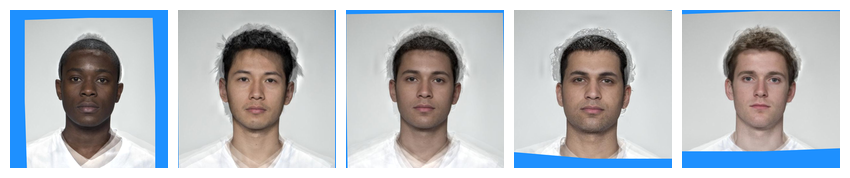
\includegraphics{index_files/figure-latex/procrustes-1.pdf}

\hypertarget{masking}{%
\subsubsection{Masking}\label{masking}}

(effect in masc paper)

\hypertarget{averaging-2}{%
\subsubsection{Averaging}\label{averaging-2}}

Texture/no

\hypertarget{symmetrising}{%
\subsubsection{Symmetrising}\label{symmetrising}}

How this is different from LL/RR mirroring.

\hypertarget{sexual-dimorphism-transform}{%
\subsubsection{Sexual dimorphism transform}\label{sexual-dimorphism-transform}}

Continuum

\hypertarget{self-resemblance-transform}{%
\subsubsection{Self-resemblance transform}\label{self-resemblance-transform}}

\hypertarget{discussion}{%
\section{Discussion}\label{discussion}}

\begin{itemize}
\tightlist
\item
  head position in 2D images

  \begin{itemize}
  \tightlist
  \item
    morphometics
  \item
    facefuns
  \end{itemize}
\item
  Natural vs standardised source images

  \begin{itemize}
  \tightlist
  \item
    right image for the question
  \end{itemize}
\item
  Averaging is N=1
\end{itemize}

\newpage

\hypertarget{references}{%
\section{References}\label{references}}

We used R {[}Version 4.0.2; R Core Team (2020){]} and the R-packages \emph{papaja} {[}Version 0.1.0.9997; Aust and Barth (2020){]}, and \emph{webmorph} {[}Version 0.0.0.9001; DeBruine (2020){]} to produce this manuscript.

\begingroup
\setlength{\parindent}{-0.5in}
\setlength{\leftskip}{0.5in}

\hypertarget{refs}{}
\begin{CSLReferences}{1}{0}
\leavevmode\hypertarget{ref-R-papaja}{}%
Aust, F., \& Barth, M. (2020). \emph{{papaja}: {Create} {APA} manuscripts with {R Markdown}}. Retrieved from \url{https://github.com/crsh/papaja}

\leavevmode\hypertarget{ref-R-webmorph}{}%
DeBruine, L. (2020). \emph{Webmorph: Morph faces}. Retrieved from \url{https://github.com/facelab/webmorph}

\leavevmode\hypertarget{ref-Gronenschild_2009}{}%
Gronenschild, E. H. B. M., Smeets, F., Vuurman, E. F. P. M., Boxtel, M. P. J. van, \& Jolles, J. (2009). The use of faces as stimuli in neuroimaging and psychological experiments: A procedure to standardize stimulus features. \emph{Behavior Research Methods}, \emph{41}, 1053--1060. \url{https://doi.org/10.3758/BRM.41.4.1053}

\leavevmode\hypertarget{ref-R-base}{}%
R Core Team. (2020). \emph{R: A language and environment for statistical computing}. Vienna, Austria: R Foundation for Statistical Computing. Retrieved from \url{https://www.R-project.org/}

\leavevmode\hypertarget{ref-CFD_2015}{}%
The chicago face database: A free stimulus set of faces and norming data. (2015). \emph{Behavior Research Methods}, \emph{47}, 1122--1135. \url{https://doi.org/10.3758/s13428-014-0532-5}

\end{CSLReferences}

\endgroup


\end{document}
